% ----------------------------------------------------------
% The RI5cy Study Case
% ----------------------------------------------------------
\chapter{The RI5CY Study Case}

The algorithm to generate Pipeline Properties, proposed in Chap.~\ref{chapter:algorithm},  was evaluated with a case study for the RI5CY processor core. RI5CY is a 4-stage pipeline processor core based on the RISC-V architecture. Its implementation is open-source and powered by PULP Platform \cite{pulp}.

For this case study, a \textit{SystemC-PPA-compliant} \cite{paper-pdd} model for the chosen core was implemented as a sequential CPU model. The properties were then automatically generated using DeSCAM \cite{descam}. From these automatically generated properties, the Pipeline Properties were finally created using the merging Pipeline Algorithm. 

This chapter starts with a brief discussion about the RISC-V Implementation Set Architecture in Sec.~\ref{section:riscv} and the RI5CY processor core in Sec.~\ref{section:ri5cy_core}. Next, the ESL implementation compliant to the \textit{SystemC-PPA} specification is detailed in Sec.~\ref{section:ri5cy_esl}. Then, the DeSCAM generated properties are presented in Sec.~\ref{section:ri5cy_micro_ppt}, followed by the Pipeline Properties in Sec.~\ref{section:ri5cy_pipe_ppt}, and finally the S2QED Properties Sec.~\ref{section:ri5cy_s2qed_ppt}.

\section{RIVC-V ISA Overview}
\label{section:riscv}
Instruction Set Architecture (ISA), as the name suggests, is the set of instructions that a computer, or more specifically a processor core, can execute. Among other things, an ISA specification will determine which operations the processor can perform, how the memory is addressed and the type and size of the instruction operands \cite{book-comp-arch}.

A Reduced Instruction Set Computer (RISC) is a computer that has a small set of instructions. These instructions have a simple fixed length encoding, and they take similar number of \textit{clock} cycles to execute \cite{book-comp-arch}. Some examples of RISC architectures are AMRv7, MIPS and RISC-V.

RISC-V is an open ISA that offers both a small base integer ISA that can be used by itself, and optional standard extensions. As an open and free to use architecture, it was initially intended to support computer architecture research and education \cite{spec-riscv}. Even so, its popularity increased rapidly and there are open-source simulators, compilers, debuggers and implementations in Hardware Description Language (HDL) for RISC-V available \cite{book-comp-org}. One of these open-source implementations is the RI5CY processor powered by PULP Platform \cite{pulp}. This implementation is used as case study in the present work and some important details are presented in the next section. 

\section{The RI5CY Processor Core}
\label{section:ri5cy_core}

RI5CY is a processor core implementation based on the RISC-V ISA. It is an in-order \textit{32 bits} core and has a pipeline with 4 stages. Besides the support for the \textit{RV32I} Base Integer Instruction Set, it has also support for the \textit{RV32C} Standard Extension for Compressed Instructions and \textit{RV32M} Integer Multiplication and Division Instruction Set Extension, and optional support for \textit{RV32F} Single Precision Floating Point Extensions. This core also implements the following PUPL specific extensions:  Post-Incrementing load and stores, Multiply-Accumulate extensions, ALU extensions, and Hardware Loops.

However, this case study is focused on the \textit{32bits} Integer Base Instructions set \textcolor{red}{[maybe some standard extensions if time allows it]} as detailed in Sec.~\ref{section:ri5cy_esl} of this chapter. Before that, however, some aspects of the pipeline, memory protocol and Load-Store Unit of the RI5CY core are briefely discussed. These implementation aspects are important for the understanding of the ESL model and for the property generation as well.

For detailed information about all the RI5CY implemented extensions, the reader can refer to the RI5CY User Manual \cite{manual-ri5cy}.

\subsection*{RI5CY Pipeline}

As aforementioned, this core implements a 4-stages pipeline: instruction fetch ($IF$), instruction decode ($ID$), execute ($EX$) and write-back ($WB$). However, most of the instructions in the base integer set, like arithmetic and logic operations, uses only the first three stages. The $WB$ stage is used, for example, when loading data from the data memory. Fig.~\ref{fig:ri5cy_pipeline} depicts the pipeline structure and its main signals.

\begin{figure}[htb!]
	\centering
	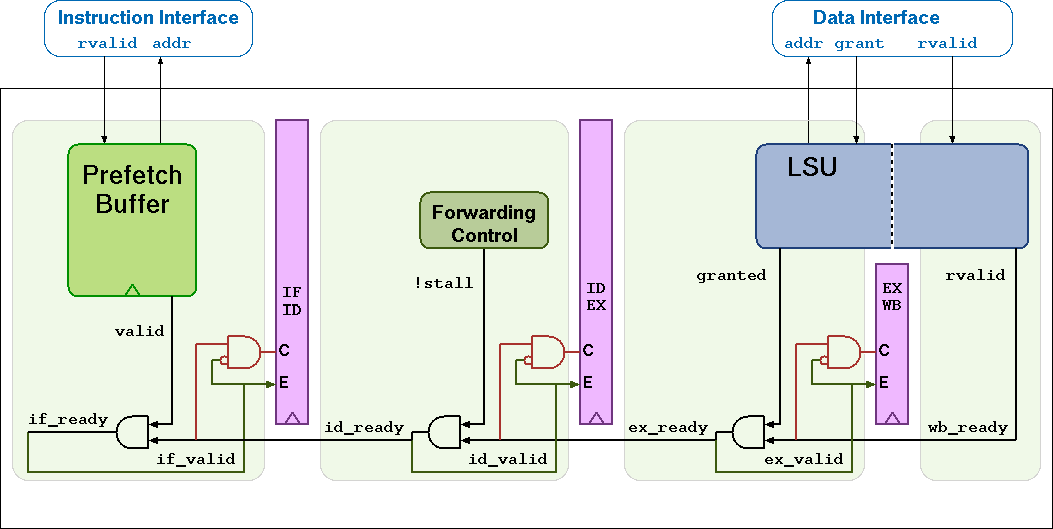
\includegraphics[width=\textwidth]{images/ri5cy_pipeline.png}
	\caption{RI5CY pipeline diagram \cite{manual-ri5cy}.}
	\label{fig:ri5cy_pipeline}
\end{figure}

The ready signal of each stage propagates from right to left and are used to inform the previous stage that the current stage is ready to operate. In this sense, each stage can finish its execution independently from the previous, but they cannot propagate (stall) if the next one is not ready. 

\subsection*{RI5CY Load-Store Unit}

The Load-Store Unit (LSU) is the component of the core responsible to access the data memory. As shown in Fig.~\ref{fig:ri5cy_pipeline}, the LSU belongs to two pipeline stages: $EX$ and $WB$. It means that a request to the data memory is sent already in the $EX$ stage. To illustrate this behaviour better, consider a LOAD instruction in the ID stage. In the next \textit{clock} cycle, the access address is computed in the $EX$ stage, and the LSU sends a request to the data memory in the same cycle. When the data arrives from memory, the LSU will write it to the correspondent register in the $WB$ stage. The memory access protocol is detailed next.

\subsection*{RI5CY Memory Access Protocol}

In order to access the data memory, the LSU sets the output address with the right address and sends a request signal. The LSU waits for a grant signal from the memory that can come in the same \textit{clock} cycle as the request or any number of \textit{clock} cycles later. After receiving the grant signal, the LSU can optionally change the outputs and make a new request or just set the request signal to low. If it was a read from memory request, e.g. LOAD instruction, the memory will send the data along with a valid signal one or more \textit{clock} cycles after the grant signal. All the LSU signals can be found on Table~\ref{tab:lsu-signals} with a brief description. 

\begin{table*}[htb!] 
	\centering 
	\caption{LSU port signals of RI5CY processor\cite{manual-ri5cy}.} 
	\label{tab:lsu-signals}
	\begin{tabular}{l|c|p{7cm}} 
		\multicolumn{1}{c}{\bfseries Signal} & \multicolumn{1}{c}{\bfseries Port Direction} & \multicolumn{1}{c}{\bfseries Description} \\     
		\hline	
		$data\_req\_o$  &  output & Request ready, must stay high until $data\_gnt\_i$ is        high for one cycle \\
		\hline
		$data\_addr\_o$[31:0]  &  output & Address \\
		\hline
		$data\_we\_o$  &  output & Write Enable, high for writes, low for reads. Sent            together with $data\_req\_o$ \\
		\hline
		$data\_wdata\_o$[31:0]  &  output & Data to be written to memory, sent together with     $data\_req\_o$ \\
		\hline
		$data\_rdata\_i$[31:0]  &  input & Data read from memory \\
		\hline
		$data\_rvalid\_i$  &  input & $data\_rdata\_i$ holds valid data when                     $data\_rvalid\_i$ is high. This signal will be high for exactly one cycle per        request. \\
		\hline
		$data\_gnt\_i$  &  input & The other side accepted the request. $data\_addr\_o$ may     change in the next cycle \\
		\hline
	\end{tabular} 
\end{table*}

The instruction memory access performed by the instruction fetcher of the core is similar to the data memory protocol. The only difference is that that the instruction fetcher does not have any writing interface, since the instruction memory is only read by the core. The instruction fetcher signals are presented on Table~\ref{tab:imem-signals}.

\begin{table*}[htb!] 
	\centering 
	\caption{Instruction memory port signals of RI5CY processor \cite{manual-ri5cy}.} 
	\label{tab:imem-signals}
	\begin{tabular}{l|c|p{7cm}} 
		\multicolumn{1}{c}{\bfseries Signal} & \multicolumn{1}{c}{\bfseries Port Direction} & \multicolumn{1}{c}{\bfseries Description} \\     
		\hline	
		$instr\_req\_o$  &  output & Request ready, must stay high until $instr\_gnt\_i$ is high for one cycle \\
		\hline
		$instr\_addr\_o$[31:0]  &  output & Address \\
		\hline
		$instr\_rdata\_i$[31:0]  &  input & Data read from memory \\
		\hline
		$instr\_rvalid\_i$  &  input & $instr\_rdata\_i$ holds valid data when $instr\_rvalid\_i$ is high. This signal will be high for exactly one cycle per request. \\
		\hline
		$instr\_gnt\_i$  &  input & The other side accepted the request. $instr\_addr\_o$ may change in the next cycle \\
		\hline
	\end{tabular} 
\end{table*}

\section{RI5CY ESL Implementation}
\label{section:ri5cy_esl}

\section{The DeSCAM Properties}
\label{section:ri5cy_micro_ppt}

\section{The Pipeline Properties}
\label{section:ri5cy_pipe_ppt}

\section{The S2QED Properties}
\label{section:ri5cy_s2qed_ppt}